\documentclass{article}
\usepackage{geometry}
\usepackage{parskip}
\usepackage[colorlinks=true]{hyperref}
\usepackage{framed}
\usepackage{listings}

\title{Anamoly/Outlier Detection}
\author{Dr. M. Kamakshaiah \\ \small{kamakshaiah.m@gmail.com}}

\date{}

\usepackage{Sweave}
\begin{document}
\Sconcordance{concordance:anadetect.tex:anadetect.Rnw:%
1 12 1 1 0 48 1 1 2 1 0 3 1 4 0 1 2 2 1 1 2 1 0 1 1 2 2 4 0 1 2 2 1 1 2 %
1 0 1 6 4 0 1 1 6 0 1 2 2 1 1 2 5 0 1 2 6 1 1 40 42 0 1 2 4 1 1 2 7 0 1 %
2 2 1 1 2 5 0 1 2 3 1 1 2 1 0 1 1 12 0 1 2 2 1 1 2 5 0 1 2 3 1 1 2 8 0 %
1 2 2 1 1 2 1 0 1 2 10 0 1 3 4 1 1 2 5 0 1 2 2 1 1 2 7 0 1 2 2 1 1 2 20 %
0 1 2 33 1 1 2 1 0 2 1 4 0 1 2 9 1 1 19 21 0 1 2 3 1 1 2 1 0 1 1 7 0 1 %
2 5 1 1 17 19 0 1 2 3 1 1 2 5 0 1 2 2 1 1 2 1 0 1 1 12 0 1 2 5 1}

\maketitle
\newpage
\tableofcontents
\newpage

\section{Introduction}

\subsection{What is Anamoly?}

In data mining, anomaly detection (also outlier detection) is the identification of rare items, events or observations which raise suspicions by differing significantly from the majority of the data. Typically the anomalous items will translate to some kind of problem such as bank fraud, a structural defect, medical problems or errors in a text. Anomalies are also referred to as outliers, novelties, noise, deviations and exceptions. \footnote{Retrieved from \url{https://en.wikipedia.org/wiki/Anomaly_detection}} 

\subsection{Confidence Interval/Level}

Anamolies are usually found using a novel concept in statistics known as Confidence Interval (CI). Confidence interval is a type of interval estimate, computed from the statistics of the observed data, that might contain the true value of an unknown population parameter. The interval has an associated \emph{Confidence Level} (CL) that, loosely speaking, quantifies the level of confidence that the parameter lies in the interval. More strictly speaking, the confidence level represents the frequency (i.e. the proportion) of possible confidence intervals that contain the true value of the unknown population parameter. In other words, if confidence intervals are constructed using a given confidence level from an infinite number of independent sample statistics, the proportion of those intervals that contain the true value of the parameter will be equal to the confidence level.

The CI is usually requires a $\mu$ and $Z$ and $\sigma$. Given all the parameters it can be represented as follows:

\begin{equation}
\centering

UL = \mu + z.\sigma \\
LL = \mu - z.\sigma
\end{equation}

Usually the composite form for CI is referred to as $\mu \pm$ z.$\sigma$. 

The confidence level is designated prior to examining the data. Most commonly, the 95\% confidence level is used. However, other confidence levels can be used, for example, 90\% and 99\%. To compute outliers using CL/I it requires \emph{standard normal variate} (Z) at given CL. The following are Z values for various standard or empirical CLs'. 


\begin{table}[h]
\centering 
\begin{tabular}{l|c} \hline
C & Z \\ \hline
99\%	& 2.576 \\
98\%	& 2.326 \\
95\%	& 1.96 \\
90\%	& 1.645 \\ \hline


\end{tabular}

\end{table}

\subsection{Outlier Dection using UDF}\footnote{UDF: User Defined Functions}

Let us see outlier detection using \emph{normal distribution}. \texttt{rnorm()} helps in simulating random data from normal distribution. For more details use \texttt{help("rnorm")} in console. 

\begin{Schunk}
\begin{Sinput}
> set.seed(123)
> x <- rnorm(100)
> par(mfrow = c(2, 1))
> plot(x); hist(x, freq = FALSE); lines(density(x), col = "red")
\end{Sinput}
\end{Schunk}
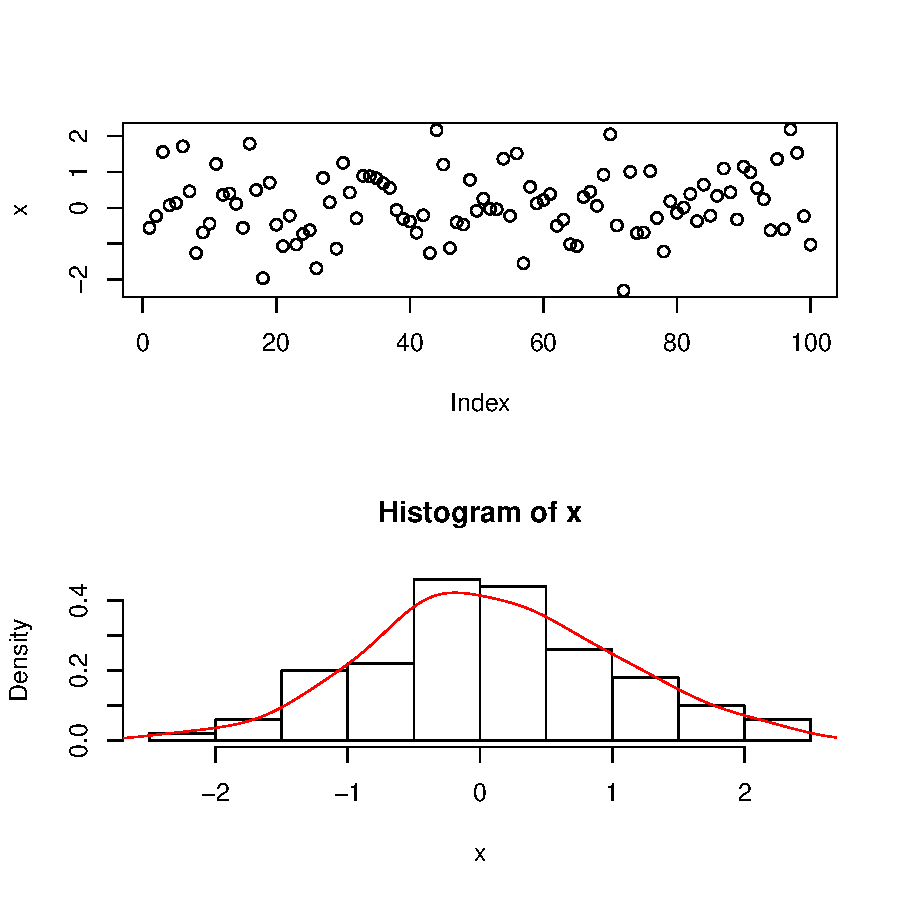
\includegraphics{anadetect-001}

From the figure it is clear that the data represents \emph{normal distribution}. Slightly skewed but acceptable. To identify outliers or anomalies; it requires to know level of confidence also known as CL. Suppose to identify outliers at 95\% CL we need to use 1.96 as multiplier in the formula. 

\begin{Schunk}
\begin{Sinput}
> ul <- mean(x) + 1.96 * sd(x)
> ll <- mean(x) - 1.96 * sd(x)
> xc <- length(x) - 10 
> plot(x, type = "l"); abline(h = ul, col = "green"); abline(h=ll, col = "green"); abline(h=mean(x), col = "red"); text(xc, ul, paste("UL=", round(ul, 2))); text(xc, ll, paste("LL=", round(ll, 2)))
\end{Sinput}
\end{Schunk}
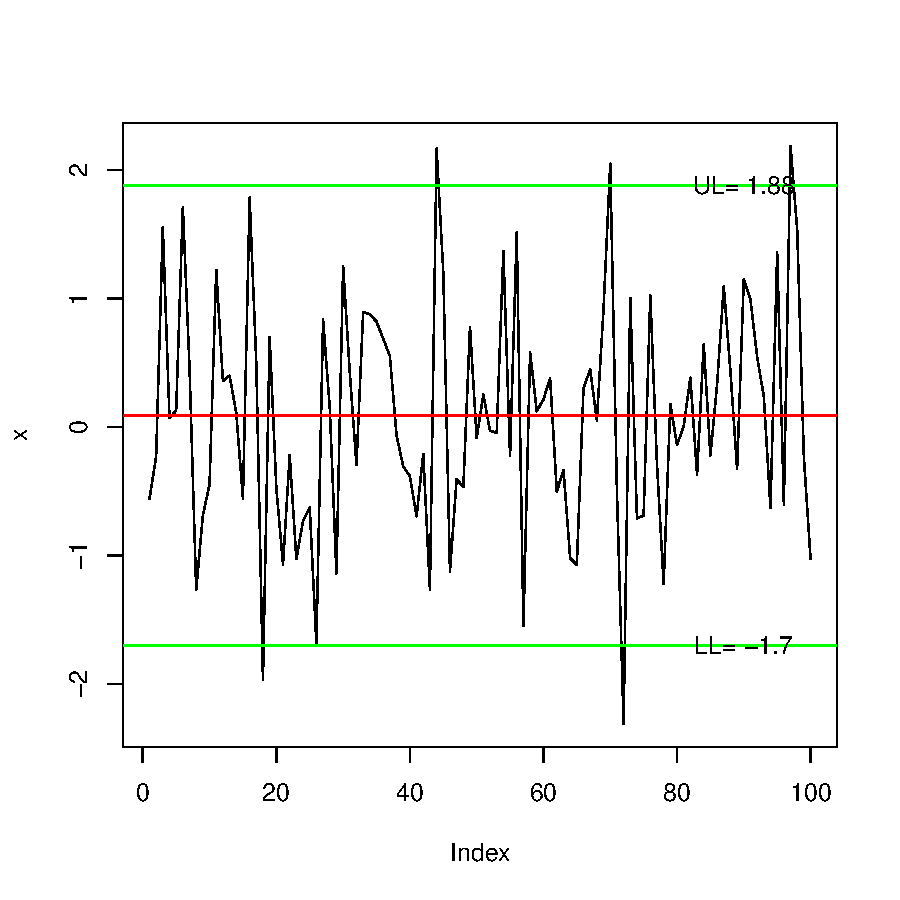
\includegraphics{anadetect-002}

Finding anamolies or outliers at 95\% CL, as we know z value at 95\% confidennce interval is 1.96. 

\begin{Schunk}
\begin{Sinput}
> y <- matrix(NA, length(x), 1)
> for (i in 1:length(x)){
+   if (x[i] <= ll | x[i] >= ul){
+   y[i] <- x[i]
+ }
+ }
> y[!is.na(y)]
\end{Sinput}
\begin{Soutput}
[1] -1.966617  2.168956  2.050085 -2.309169  2.187333
\end{Soutput}
\end{Schunk}

There are 5 outliers in data. Below graph adds visualization to the outliers. 

\begin{Schunk}
\begin{Sinput}
> plot(x, type = "l"); points(y, col = "red", pch = 19)
\end{Sinput}
\end{Schunk}
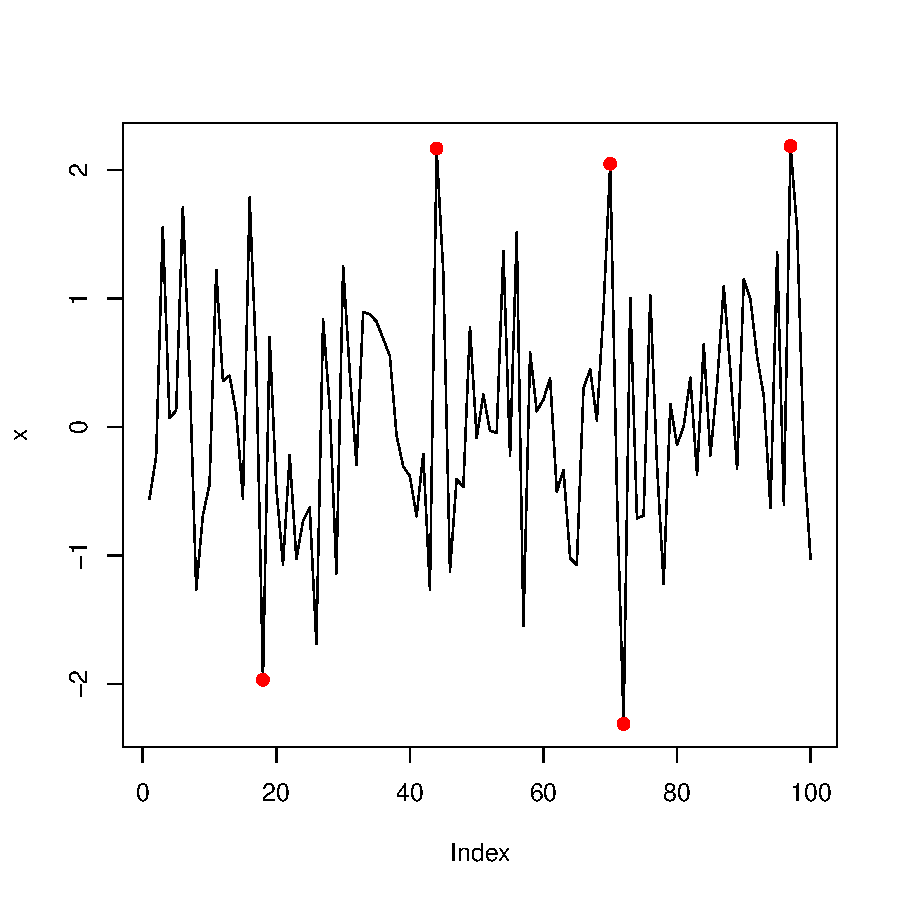
\includegraphics{anadetect-004}

\subsubsection{Testing}

Let us sumup all the above code as in the form of function. 


\begin{leftbar}
\begin{Schunk}
\begin{Sinput}
> outliers <- function(x, cl = 0.95, plot = TRUE, out = FALSE, na.remove = FALSE, complete = FALSE){
+   
+   # Missing data treatment, considered as outliers
+   if (na.remove == TRUE){
+     for (i in 1:length(x)){
+       if(is.na(x[i])){
+         x[i] <- 0
+       }
+     }
+   } else if (complete == TRUE){
+     x <- complete.cases(x)
+   }
+   
+   z <- -qnorm((1-cl)/2)
+   
+   ul <- mean(x) + z * sd(x)
+   ll <- mean(x) - z * sd(x)
+   
+   
+   xc <- length(x) - quantile(x, 0.1) 
+   y <- matrix(NA, length(x), 1)
+   
+   for (i in 1:length(x)){
+     if (x[i] <= ll | x[i] >= ul){
+       y[i] <- x[i]
+     }
+   }
+   
+   if(out == TRUE){
+     print(y[!is.na(y)])  
+   }
+   
+   
+   if(plot == TRUE){
+     plot(x, type = "l"); points(y, col = "red", pch = 19); abline(h = ul, col = "green"); abline(h=ll, col = "green"); abline(h=mean(x), col = "red"); text(xc, ul, paste("UL=", round(ul, 2))); text(xc, ll, paste("LL=", round(ll, 2)))
+     
+   }  
+   
+ }
\end{Sinput}
\end{Schunk}
\end{leftbar} 


Now it is time to test the code:

\begin{Schunk}
\begin{Sinput}
> outliers(x, out = TRUE)
\end{Sinput}
\begin{Soutput}
[1] -1.966617  2.168956  2.050085 -2.309169  2.187333
\end{Soutput}
\end{Schunk}

For plot:

\begin{Schunk}
\begin{Sinput}
> outliers(x, plot = TRUE)
\end{Sinput}
\end{Schunk}
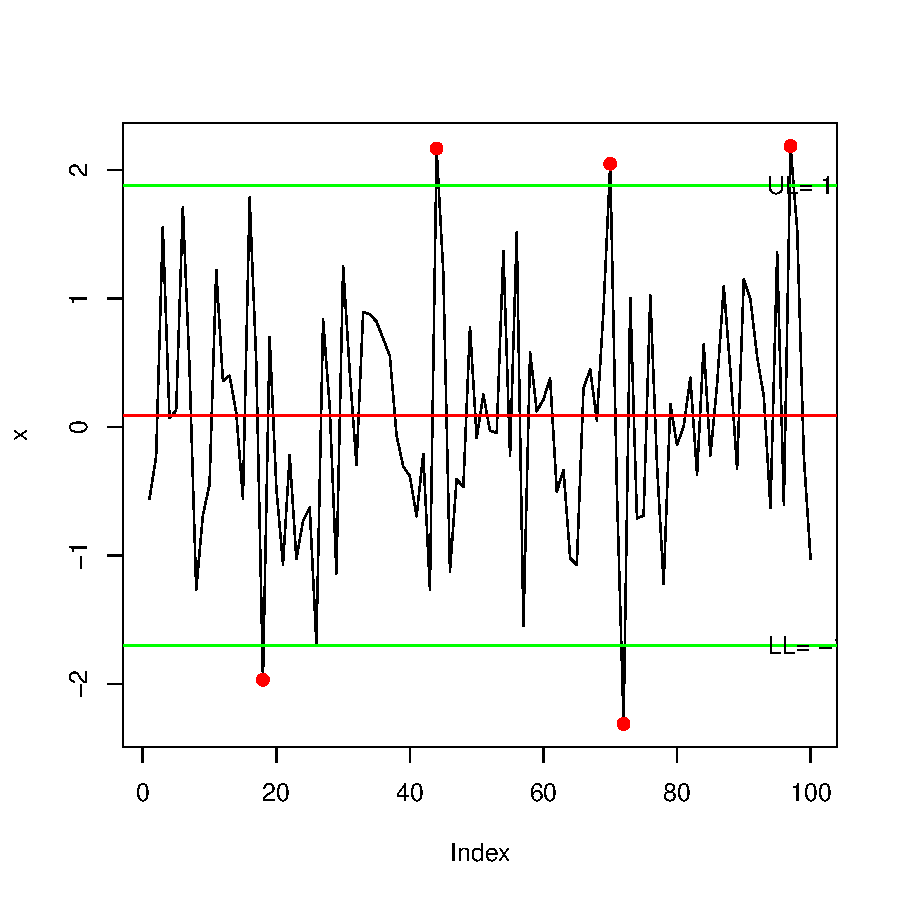
\includegraphics{anadetect-007}

\section{Testing on \emph{APPLE} data sets}


\begin{Schunk}
\begin{Sinput}
> df <- read.csv("/media/ubuntu/C2ACA28AACA27895/WORK/R/anomaly/aapl.csv")
> head(df)
\end{Sinput}
\begin{Soutput}
  X adj_close  close     date   high    low    open   volume
1 0     31.68 130.31 01/03/00 132.06 118.50 1000.00 38478000
2 1     29.66 122.00 02/03/00 127.94 120.69  127.00 11136800
3 2     31.12 128.00 03/03/00 128.23 120.00  124.87 11565200
4 3     30.56 125.69 06/03/00 129.13 125.00  126.00  7520000
5 4     29.87 122.87 07/03/00 127.44 121.12  126.44  9767600
6 5     29.66 122.00 08/03/00 123.94 118.56  122.87  9690800
\end{Soutput}
\end{Schunk}

Testing UDF \texttt{outliers()} on the APPLE data sets:

\begin{Schunk}
\begin{Sinput}
> outliers(df$adj_close, plot = TRUE)
\end{Sinput}
\end{Schunk}
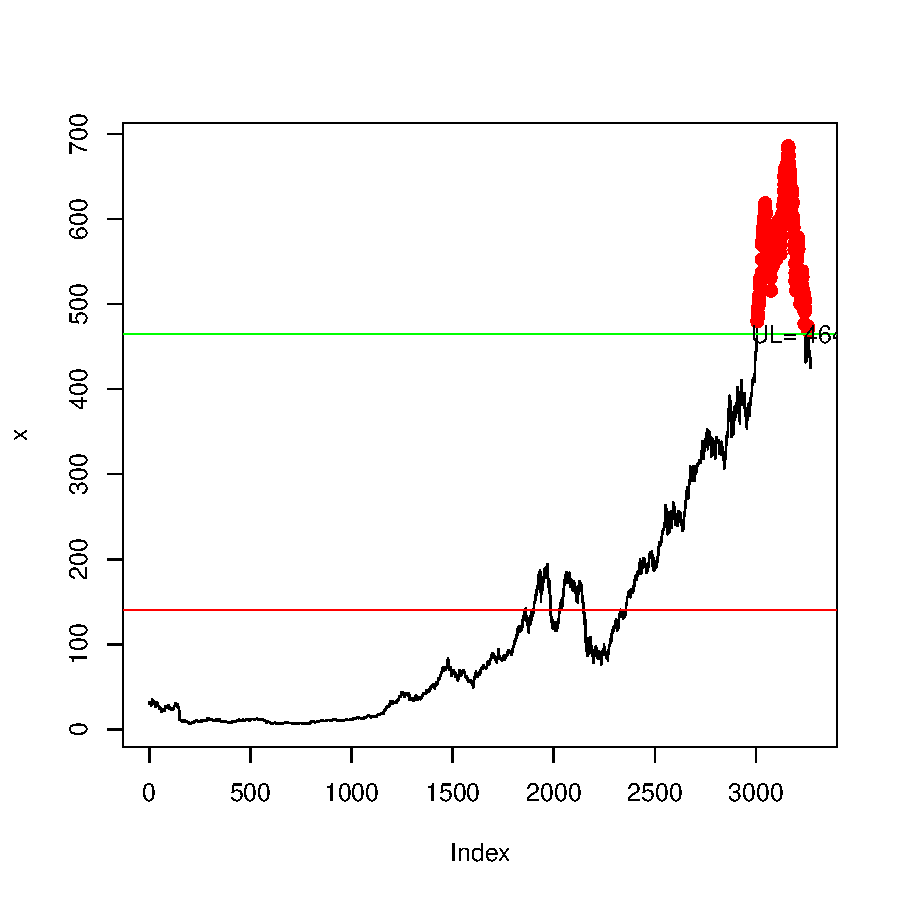
\includegraphics{anadetect-009}

Suppose we would like to know the outliers at 99.9\% CL, which is rather unusual, then we might issue arguments \texttt{cl = 0.999, out = TRUE}.


\begin{Schunk}
\begin{Sinput}
> outliers(df$adj_close, cl = 0.999, plot = TRUE, out = TRUE)
\end{Sinput}
\begin{Soutput}
[1] 685.58 685.76
\end{Soutput}
\end{Schunk}
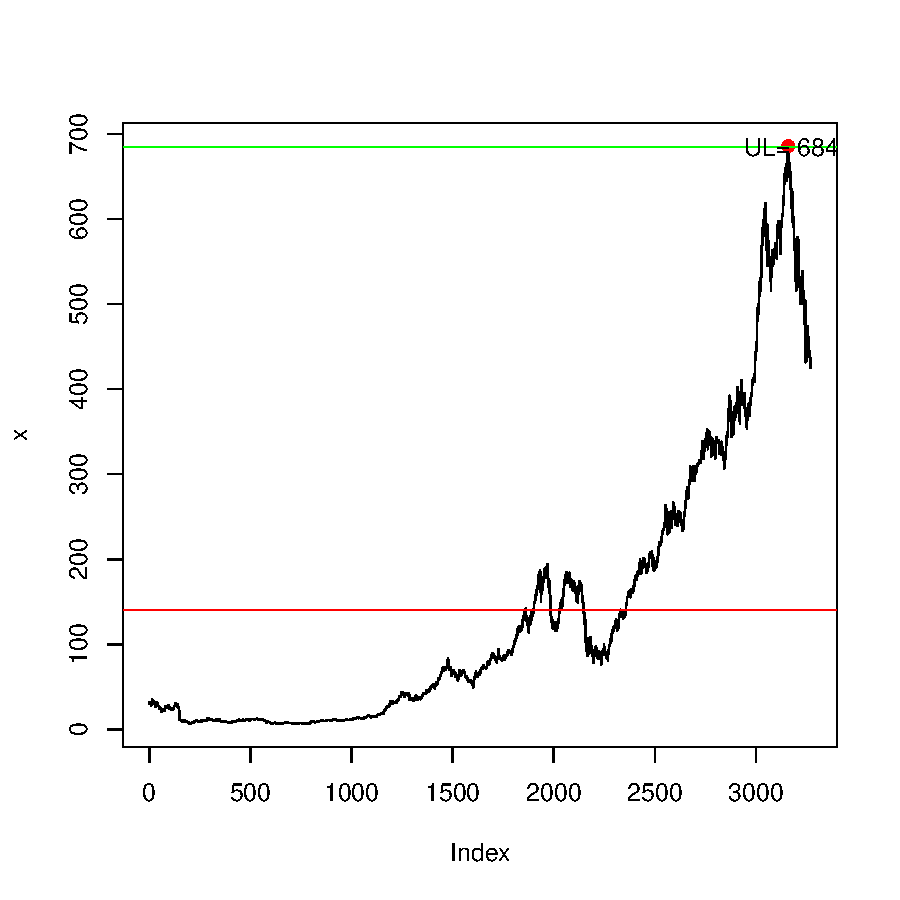
\includegraphics{anadetect-010}

As you can see the outliers are greatly reduced to two data points. This way it is possible for us to plot rest of the variables in the data set. Let us use the same parameters i.e. \texttt{cl = 0.999, out = TRUE}. 

\begin{Schunk}
\begin{Sinput}
> df <- df[, -1] # to get rid of first column
> outliers(df[, 2], cl = 0.999, plot = TRUE, out = TRUE)
\end{Sinput}
\begin{Soutput}
[1] 699.78 701.91 702.10 698.70 700.09
\end{Soutput}
\begin{Sinput}
> 
\end{Sinput}
\end{Schunk}
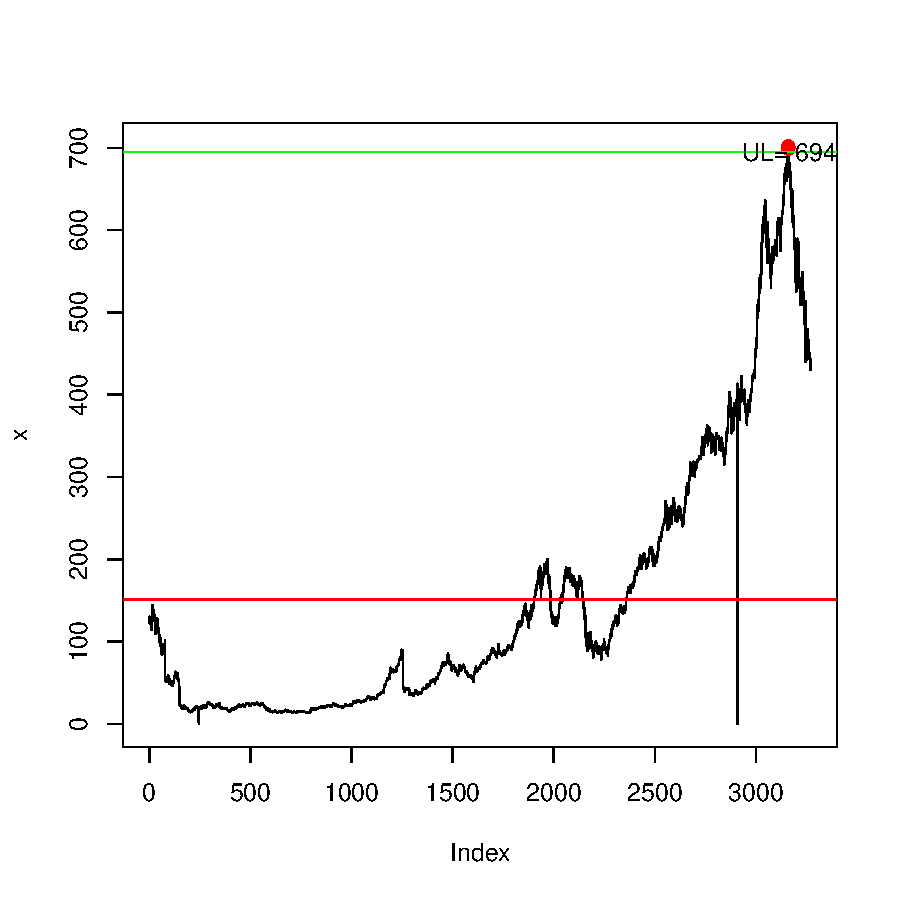
\includegraphics{anadetect-011}

The above plot is for third variable in the data i.e. \texttt{close} (closing price). Suppose we would like to plot the last variable i.e. \texttt{volume}. We might be able to use the following code. 

\subsubsection{Finding \emph{missing} data}

\begin{Schunk}
\begin{Sinput}
> outliers(complete.cases(df[, 7]))
\end{Sinput}
\end{Schunk}
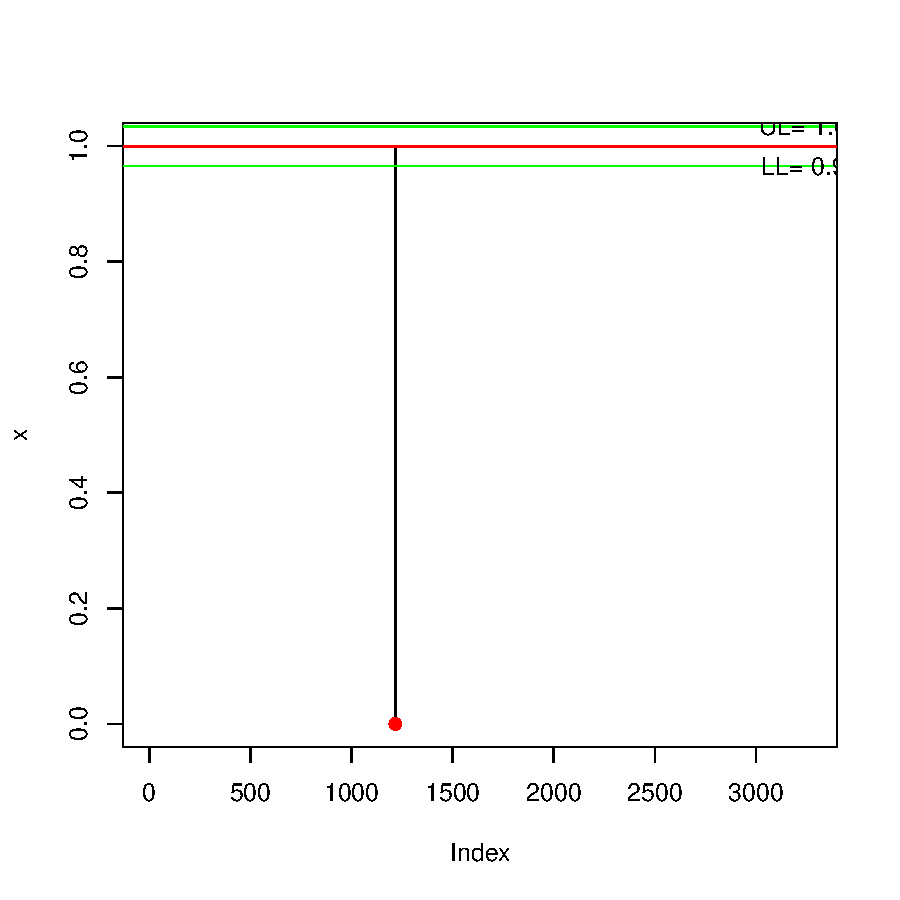
\includegraphics{anadetect-012}

This clarly shows that there is one extreme outlier in data variable \texttt{volume},  \emph{whose value is zero}, and the point is between 1000th and 1500th data points (or rows). To know the exact case of the missing data point:

\begin{Schunk}
\begin{Sinput}
> which(is.na(df[, 7]))
\end{Sinput}
\begin{Soutput}
[1] 1217
\end{Soutput}
\end{Schunk}

To retrieve all other outliers at given CL say 99.9\%: 

\begin{Schunk}
\begin{Sinput}
> outliers(df[, 7], cl = 0.99, out = TRUE, na.remove = TRUE)
\end{Sinput}
\begin{Soutput}
 [1] 265069000  86610600  72795600  66916800  61052400  62908800  63133000
 [8]  98872400  91721800  61175600  79551800  61618200  93272400  68560800
[15] 113025600  63240800  60039200  82579200  98328300  61717400  72927900
[22]  74859300  96338800  66627700  81423900  60566000  62874200  83815500
[29]  79764600  95134600  70433800  66173800  60167400  69134100 119617800
[36] 105460000  84450200  62063500  68395700  66937800  61476900  64117600
[43]  78093900  62942600  62505600  66667500  83150800  67902200  64113000
[50]  67458500  63057700  62034100  74006900  64781500  83688500  79065900
[57]  62780700  61583700  86955500 120463200  71638100  74404700  63763700
[64]  60573800  67442600  67128300  59866200  93644900  81942800  75264900
[71]  67099000  78847900  79260700  70749800  70732900  62936700  78345000
[78]  80314600  59836800  69677800  66217400  61314800  65415500  66682500
[85]  61520300  59857800  67178500
\end{Soutput}
\end{Schunk}
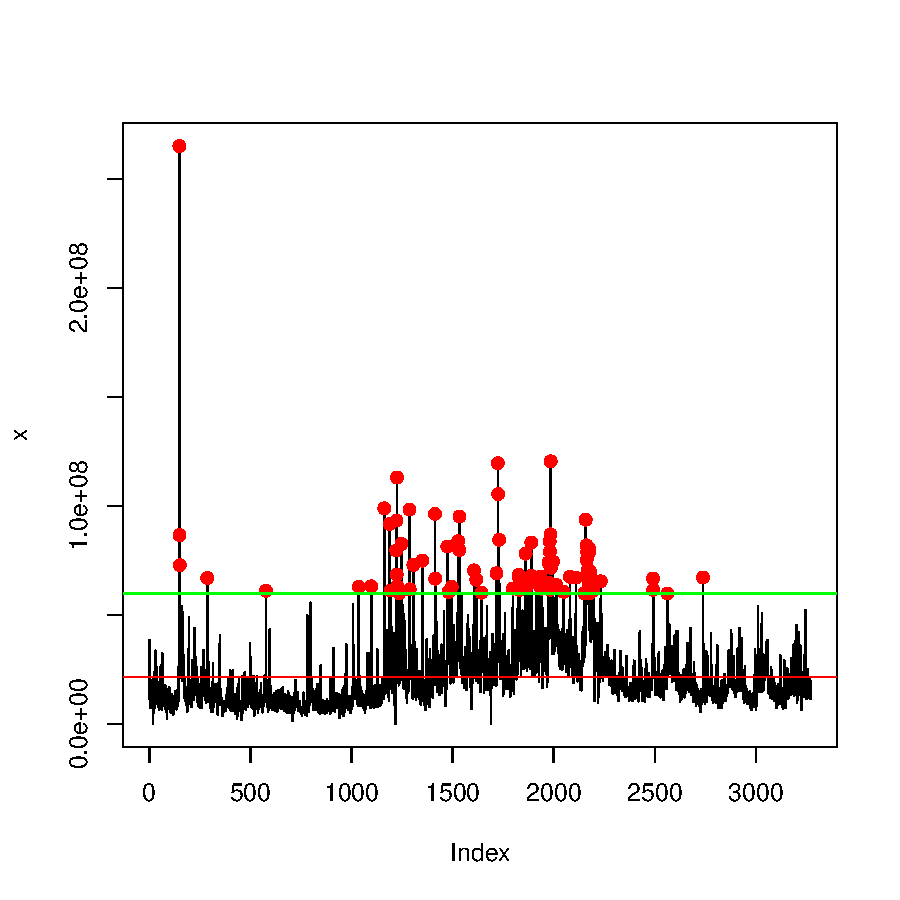
\includegraphics{anadetect-014}

Above plot doesn't show missing data but it has all those outliers defined at 99.9\% CL. 

\section{Handling Outliers in Regression}

\subsection{Simple Linear Regression}

Simple linear regression is a linear regression model with a single explanatory variable. That is, it concerns two-dimensional sample points with one independent variable and one dependent variable (conventionally, the x and y coordinates in a Cartesian coordinate system) and finds a linear function (a non-vertical straight line) that, as accurately as possible, predicts the dependent variable values as a function of the independent variables. The adjective simple refers to the fact that the outcome variable is related to a single predictor. \footnote{Retrieved from \url{https://en.wikipedia.org/wiki/Simple_linear_regression}}

Consider the model function

${y=\alpha +\beta x,}$

which describes a line with slope $\beta$ and y-intercept $\alpha$. In general such a relationship may not hold exactly for the largely unobserved population of values of the independent and dependent variables; we call the unobserved deviations from the above equation the errors. Suppose we observe n data pairs and call them {(xi, yi), i = 1, ..., n}. We can describe the underlying relationship between yi and xi involving this error term $\epsilon_{i}$ by

$y_i = \alpha + \beta x_i + \varepsilon_i.$

This relationship between the true (but unobserved) underlying parameters $\alpha$ and $\beta$ and the data points is called a linear regression model.

\subsection{Cooks Distance}

Cook's distance or Cook's D is a commonly used estimate of the influence of a data point when performing a least-squares regression analysis. In a practical ordinary least squares analysis, Cook's distance can be used in several ways: to indicate influential data points that are particularly worth checking for validity; or to indicate regions of the design space where it would be good to be able to obtain more data points. It is named after the American statistician R. Dennis Cook, who introduced the concept in 1977.

Cook's distance $D_{i}$ of observation for $i=1,\dots ,n$ is defined as the sum of all the changes in the regression model when observation $i$ is removed from it.

\begin{center}
$D_{i}={\frac {\sum _{j=1}^{n}\left({\widehat {y\,}}_{j}-{\widehat {y\,}}_{j(i)}\right)^{2}}{ps^{2}}}$
\end{center}

where ${\widehat {y\,}}_{j(i)}$ is the fitted response value obtained when excluding $i$, and ${\displaystyle s^{2}\equiv \left(n-p\right)^{-1}\mathbf {e} ^{\top }\mathbf {e} }$ is the mean squared error of the regression model.
 
Using simulations. 

{
\begin{Schunk}
\begin{Sinput}
> fit <- lm(x ~ ., data = as.data.frame(x))
> cd <- cooks.distance(fit)
> plot(cd); abline(h = 4*mean(cd, na.rm = T), col ="red"); text(x = 1:length(cd)+1, y = cd, labels = ifelse(cd > 4*mean(cd, na.rm = T), names(cd), ""), col = "red")
\end{Sinput}
\end{Schunk}
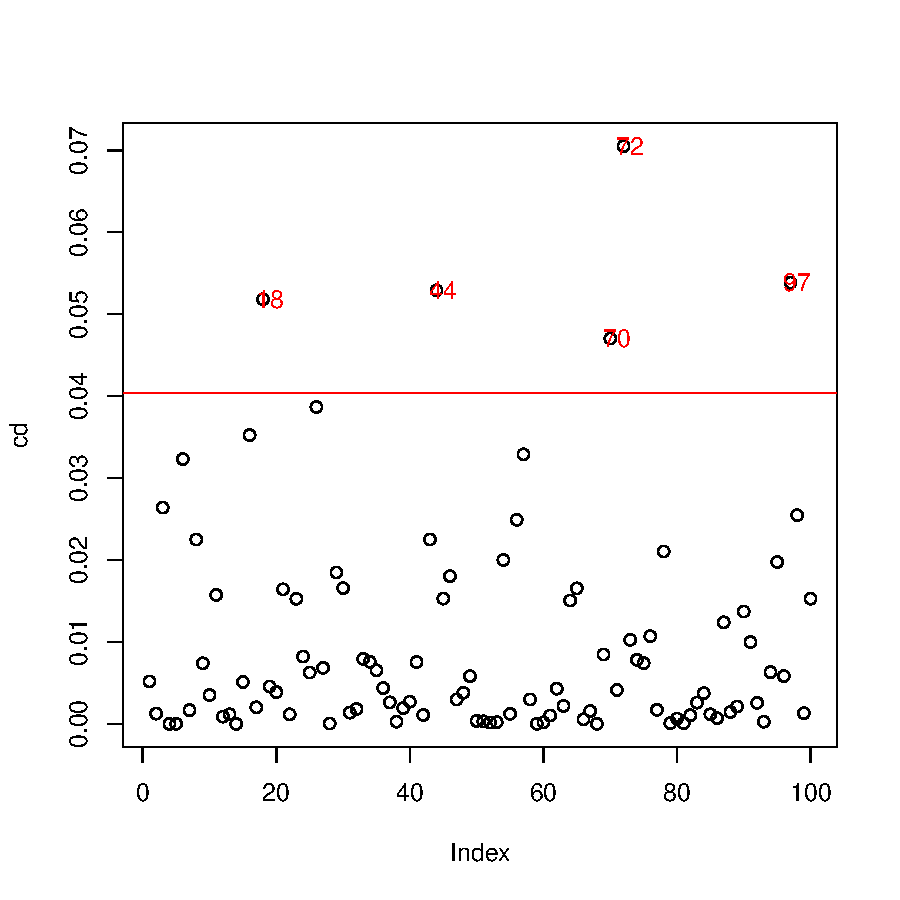
\includegraphics{anadetect-015}
\\
\begin{center}
Figure 1: Outliers through Cooks Distance
\end{center}

}

Let us create a function for the same. 

\begin{leftbar}
\begin{Schunk}
\begin{Sinput}
> cookOutliers <- function(x, result = FALSE, plot = FALSE){
+   
+   
+   fit <- lm(x ~ ., data = as.data.frame(x))
+   cd <- cooks.distance(fit)
+   
+   out <- list(desc = summary(fit), outliers = cd[cd > 4*mean(cd, na.rm = T)])
+   
+   if (result){
+     return(list(desc = summary(fit), outliers = cd[cd > 4*mean(cd, na.rm = T)]))
+   } 
+   
+  if (plot){
+    plot(cd); abline(h = 4*mean(cd, na.rm = T), col ="red"); text(x = 1:length(cd)+1, y = cd, labels = ifelse(cd > 4*mean(cd, na.rm = T), names(cd), ""), col = "red")
+    
+  }
+    
+ }
\end{Sinput}
\end{Schunk}
\end{leftbar}

To get the outliers use

\begin{Schunk}
\begin{Sinput}
> out <- cookOutliers(x, result = TRUE)
> out$outliers
\end{Sinput}
\begin{Soutput}
        18         44         70         72         97 
0.05181334 0.05290348 0.04702546 0.07050693 0.05384308 
\end{Soutput}
\end{Schunk}

These points are the outliers in the above Figure 1. 

\subsection{Using CI in Regression}

\begin{leftbar}
\begin{Schunk}
\begin{Sinput}
> regOutliers <- function(x = rnorm(100), y= rnorm(100), newdf=as.data.frame(seq(min(x), max(x), length.out = 100)), ci = 0.999, plot = FALSE, out = FALSE){
+   
+   fit <- lm(y ~ x, data = cbind.data.frame(x, y))
+   
+   conf_int <- predict(fit, newdf, interval = "confidence", level = ci)
+   
+   if(plot){
+     plot(x, y, xlab="x", ylab="y", main="Regression"); text(x+0.2, y, row.names(cbind.data.frame(x, y)), cex = 0.5, col = "red")
+     abline(fit, col="red")
+     matlines(newdf, conf_int[,2:3], col = "blue", lty=2)
+     
+   }
+   if(out){
+     return(conf_int)
+   }
+ }
\end{Sinput}
\end{Schunk}
\end{leftbar}

Testing 

\begin{Schunk}
\begin{Sinput}
> regOutliers(plot = TRUE)
\end{Sinput}
\end{Schunk}
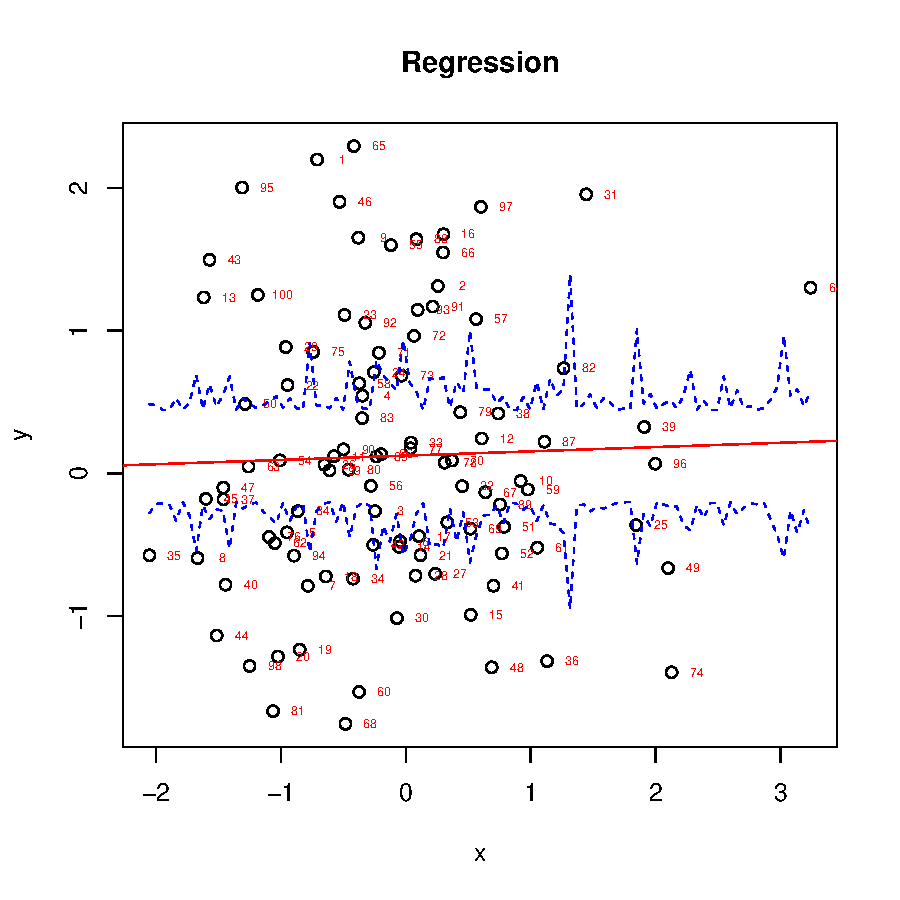
\includegraphics{anadetect-019}

In case if you are interested you can try with other data. For results/output try:

\begin{Schunk}
\begin{Sinput}
> out <- regOutliers(rnorm(100), rnorm(100), 0.999, out = TRUE)
> head(out)
\end{Sinput}
\begin{Soutput}
         fit        lwr       upr
1 0.11546744 -0.2627299 0.4936647
2 0.10940869 -0.2337684 0.4525858
3 0.07659465 -0.5436176 0.6968069
4 0.10389312 -0.2351903 0.4429765
5 0.10281492 -0.2387721 0.4444019
6 0.07372656 -0.5898855 0.7373386
\end{Soutput}
\end{Schunk}

\section{Conclusion}

At present this module support three functions viz., \texttt{outliers()}, \texttt{CookOutliers()} and \texttt{regOutliers()}. All functions supports confidence intervals and issues a plot by choice. In future development more advanced analysis will be provided. 

\end{document}
